\documentclass[twoside,11pt]{article}

% Any additional packages needed should be included after jmlr2e.
% Note that jmlr2e.sty includes epsfig, amssymb, natbib and graphicx,
% and defines many common macros, such as 'proof' and 'example'.
%
% It also sets the bibliographystyle to plainnat; for more information on
% natbib citation styles, see the natbib documentation, a copy of which
% is archived at http://www.jmlr.org/format/natbib.pdf

\usepackage{jmlr2e}
\usepackage{doi}

\usepackage{subcaption}
\usepackage{url}
\usepackage{color}
\usepackage{listings}
\usepackage{amsmath}
\usepackage{tikz}
\usetikzlibrary{bayesnet}

% Definitions of handy macros can go here

% Heading arguments are {volume}{year}{pages}{submitted}{published}{author-full-names}

\jmlrheading{?}{2014}{?-?}{?/??}{?/??}{Jaakko Luttinen}

% Short headings should be running head and authors last names

\ShortHeadings{BayesPy: Variational Bayesian Inference in Python}{Luttinen}
\firstpageno{1}

\begin{document}

\title{BayesPy: Variational Bayesian Inference in Python}

\author{\name Jaakko Luttinen \email jaakko.luttinen@aalto.fi \\
       \addr Department of Information and Computer Science\\
       Aalto University, Finland}

\editor{?}

\maketitle

\begin{abstract}%   <- trailing '%' for backward compatibility of .sty file
  BayesPy is an open-source Python software package for performing variational
  Bayesian inference.  It is based on the variational message passing framework
  and supports conjugate exponential family models.  By removing the tedious
  task of implementing the variational Bayesian update equations, the user can
  construct models faster and in a less error-prone way.  Simple syntax,
  flexible model construction and efficient inference make BayesPy suitable for
  both average and expert Bayesian users.
\end{abstract}

\begin{keywords}
  Variational Bayes, variational message passing, Python, probabilistic
  programming
\end{keywords}

\section{Introduction}

Bayesian framework provides theoretically solid and consistent way to construct
models and perform inference.  In practice, however, the inference is usually
analytically intractable and is therefore based on approximation methods such as
variational Bayes (VB), expectation propagation (EP) and Markov chain Monte
Carlo (MCMC) \citep{Bishop:2006}.  Deriving and implementing the formulas for an
approximation method is often straightforward but tedious, time consuming and
error prone.


BayesPy is a Python package providing tools for constructing Bayesian models and
performing variational Bayesian inference easily and efficiently.  It is based
on variational message passing (VMP) framework which defines a simple and local
message passing protocol \citep{Winn:2005}.  This enables implementation of small
general modules that can be used as building blocks for large complex models.
BayesPy offers a comprehensive collection of built-in blocks that can be used to
build a wide range of models and a simple interface for implementing custom
blocks.  The package is written for Python 3 and released under the GNU General
Public License v3.0 (GPLv3).


Several other projects have similar goals for making Bayesian inference easier
and faster to apply.  VB inference is available in Bayes Blocks
\citep{Raiko:2007}, VIBES \citep{Bishop:2002} and Infer.NET \citep{Infer.NET}.
Bayes Blocks is an open-source C++/Python package but it is limited to scalar
Gaussian nodes, a few deterministic functions and fully factorial posterior
approximation, thus making it very limited.  VIBES is an old software package
for Java, released under the revised BSD license, but it is no longer actively
developed.  VIBES has been replaced by Infer.NET, which supports a wide range of
posterior approximations.  However, Infer.NET is partly closed source and
licensed for non-commercial use only.  Instead of VB inference, mainly MCMC is
supported by other projects such as PyMC \citep{PyMC}, OpenBUGS \citep{OpenBUGS},
Dimple \citep{Dimple} and Stan \citep{Stan}.  Thus, there is a need for an open
source and maintained VB software package.



\section{Features}


BayesPy can be used to construct a wide range of conjugate exponential family
models.  The documentation provides detailed examples of how to construct, for
instance, regression models, principal component analysis models, linear
state-space models, mixture models and hidden Markov models.  In addition,
BayesPy has been used in two publications about parameter expansion and
time-varying dynamics for linear state-space models
\citep{Luttinen:2013,Luttinen:2014}, which show that it is applicable to large
complex models requiring efficient inference.



Using BayesPy for Bayesian inference consists of four main steps: constructing
the model, providing data, finding the posterior approximation and examining the
results.  The user constructs the model from small modular blocks called nodes.
Roughly, each node corresponds to a latent variable, a set of observations or a
deterministic function.  Some of the nodes may be set as observed by providing
data.  After that, inference engine is initialized and the message passing
algorithm is run in order to obtain the posterior approximation.  The resulting
posterior can be examined, for instance, by using a few built-in plotting
functions or printing the parameters of the posterior distributions.


Nodes are the key part of BayesPy as they are used to construct the model.
There are two types of nodes in BayesPy: stochastic and deterministic.
Stochastic nodes correspond to probability distributions and deterministic nodes
correspond to functions.  Built-in stochastic nodes include all common
exponential family distributions (e.g., Gaussian, gamma, Dirichlet and Poisson
distributions), a general mixture distribution and a few complex nodes for
dynamic variables (e.g., discrete and Gaussian Markov chains).  Built-in
deterministic nodes include a gating node and a general sum-product node.  In
case a model cannot be constructed using the built-in nodes, the documentation
provides instructions for implementing new nodes.



BayesPy is designed to be simple enough for average users but flexible and
efficient enough for expert users.  One goal is to keep the syntax easy and
intuitive to read and write by making it similar to the mathematical formulation
of the model.  Missing values are easy to handle and the variables can be
monitored by plotting the posterior distributions during the learning.  BayesPy
has also preliminary support for some advanced VB methods such as stochastic
variational inference \citep{Hoffman:2013}, deterministic annealing
\citep{Katahira:2008}, collapsed inference \citep{Hensman:2012},
Riemannian-gradient-based optimization \citep{Honkela:2010}, parameter
expansions \citep{Qi:2007} and pattern searches \citep{Honkela:2003}.  For
developers, the unit testing framework helps in finding bugs, making changes and
implementing new features in a robust manner.



BayesPy can be installed similarly to other Python packages.  It requires Python
3 and a few popular packages: NumPy, SciPy, matplotlib and h5py.  The latest
release can be installed from Python Package Index (PyPI) and detailed
instructions can be found from the comprehensive online documentation
\citep{bayespy.org}.  The latest development version is available at
GitHub\footnote{\url{https://github.com/bayespy/bayespy}}, which is also the
platform used for reporting bugs and making pull requests.


%- numpy, scipy, matplotlib, h5py

%- documentation

%- installation

%- repository


%- clear syntax

%- unit tests

%- parameter expansion

%- monitoring

%- missing values

%- examples: PCA, LSSM, HMM, mixture models

%- used in two publications, \citep{Luttinen:2013, Luttinen:2014}


\section{Example}

\lstset{ %
  basicstyle=\footnotesize,        % the size of the fonts that are used for the code
  breakatwhitespace=false,         % sets if automatic breaks should only happen at whitespace
  breaklines=true,                 % sets automatic line breaking
  captionpos=b,                    % sets the caption-position to bottom
  commentstyle=\color{green},    % comment style
  deletekeywords={...},            % if you want to delete keywords from the given language
  escapeinside={\%*}{*)},          % if you want to add LaTeX within your code
  extendedchars=true,              % lets you use non-ASCII characters; for 8-bits encodings only, does not work with UTF-8
%  frame=single,                    % adds a frame around the code
  keepspaces=true,                 % keeps spaces in text, useful for keeping indentation of code (possibly needs columns=flexible)
  keywordstyle=\color{blue},       % keyword style
  morekeywords={*,...},            % if you want to add more keywords to the set
  firstnumber=last,
  numbers=left,                    % where to put the line-numbers; possible values are (none, left, right)
  numbersep=10pt,                   % how far the line-numbers are from the code
  numberstyle=\tiny\color{black}, % the style that is used for the line-numbers
  rulecolor=\color{black},         % if not set, the frame-color may be changed on line-breaks within not-black text (e.g. comments (green here))
  showspaces=false,                % show spaces everywhere adding particular underscores; it overrides 'showstringspaces'
  showstringspaces=false,          % underline spaces within strings only
  showtabs=false,                  % show tabs within strings adding particular underscores
  stepnumber=1,                    % the step between two line-numbers. If it's 1, each line will be numbered
  stringstyle=\color{orange},     % string literal style
  tabsize=2,                       % sets default tabsize to 2 spaces
%  title=\lstname,                   % show the filename of files included with \lstinputlisting; also try caption instead of title
  belowcaptionskip=1\baselineskip,
  breaklines=true,
  frame=L,
  xleftmargin=1.3\parindent,
  showstringspaces=false,
  basicstyle=\footnotesize\ttfamily,
%  keywordstyle=\bfseries\color{green!40!black},
%  commentstyle=\itshape\color{purple!40!black},
%  identifierstyle=\color{blue},
%  stringstyle=\color{orange},
  language=Python
}

\begin{figure}
  \centering
  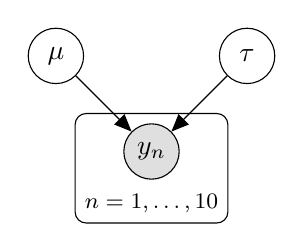
\begin{tikzpicture}
    \node [obs] (yn) {$y_n$};
    \node [latent, above left=of yn] (mu) {$\mu$};
    \node [latent, above right=of yn] (tau) {$\tau$};

    \edge {mu, tau} {yn};

    \tikzstyle{plate caption} = [caption, node distance=0, inner sep=0pt,
    below=5pt of #1.south]

    \plate {} {(yn)} {$n=1,\ldots,10$};
  \end{tikzpicture}
  \caption{Graphical model of the example problem.}
  \label{fig:graphical_model}
\end{figure}
In order to demonstrate BayesPy, this section solves an extremely simple problem
but which includes the main steps of using BayesPy.  The task is to estimate the
unknown mean and precision parameters of a Gaussian distribution given ten
observations.  Thus, the likelihood function is Gaussian:
\begin{align*}
  p(y_1,\ldots,y_{10}|\mu,\tau) &= \prod^{10}_{n=1}\mathcal{N}(y_n | \mu, \tau),
\end{align*}
where the Gaussian distribution is parameterized by precision instead of
variance.  The unknown mean $\mu$ and precision $\tau$ are given broad Gaussian
and gamma priors, respectively:
\begin{align*}
  p(\mu) &= \mathcal{N}(\mu|0, 10^{-6}), & p(\tau) &= \mathcal{G}(\tau|10^{-6},
  10^{-6}).
\end{align*}
Figure~\ref{fig:graphical_model} shows the graphical model of this simple model.
The model is constructed in BayesPy by creating nodes:
\begin{lstlisting}
from bayespy.nodes import GaussianARD, Gamma
mu = GaussianARD(0, 1e-6)
tau = Gamma(1e-6, 1e-6)
\end{lstlisting}
These two nodes represent the two unknown variables that we are interested in.
They are the parameters of the Gaussian distribution of the observed variable:
\begin{lstlisting}
y = GaussianARD(mu, tau, plates=(10,))
\end{lstlisting}
The number of observations is given as plates which define the number of
repetitions.  Note that the syntax of the model construction is similar to the
mathematical formulation which defines the conditional distributions for each
variable.  Thus, it is easy to understand the model from the Python code.  After
the model has been constructed, some nodes are marked as observed and given
data:
\begin{lstlisting}
y.observe([4.5, 3.9, 6.3, 5.6, 4.9, 2.8, 7.4, 6.1, 4.8, 2.1])
\end{lstlisting}
Next, we want to find the posterior approximation for our latent variables.  We
create the VB inference engine:
\begin{lstlisting}
from bayespy.inference import VB
Q = VB(y, mu, tau)
\end{lstlisting}
The inference engine takes all the stochastic nodes of the model as input.  The
message passing algorithm can be run by calling \texttt{update} method:
\begin{lstlisting}
Q.update(repeat=100)
\end{lstlisting}
The algorithm is run for 100 iterations or until it converges.  In this case,
the algorithm converges in four iterations.  The posterior approximation can be
examined, for instance, by plotting the probability density functions of the
latent variables:
\begin{lstlisting}
import bayespy.plot as bpplt
import numpy as np
bpplt.pyplot.figure()
bpplt.pdf(Q[mu], np.linspace(0, 10, num=300))
bpplt.pyplot.figure()
bpplt.pdf(Q[tau], np.linspace(0, 2, num=300))
bpplt.pyplot.show()
\end{lstlisting}
Figure~\ref{fig:posterior} shows the resulting approximate posterior
distributions.  The module \texttt{bayespy.plot} contains functions for simple
plotting tasks, such as plotting the probability density function or the Hinton
diagram of a variable.  Note that the standard \texttt{pyplot} module of
Matplotlib is available at the \texttt{plot} module of BayesPy.
\begin{figure}
  \begin{center}
    \begin{subfigure}[b]{0.4\textwidth}
      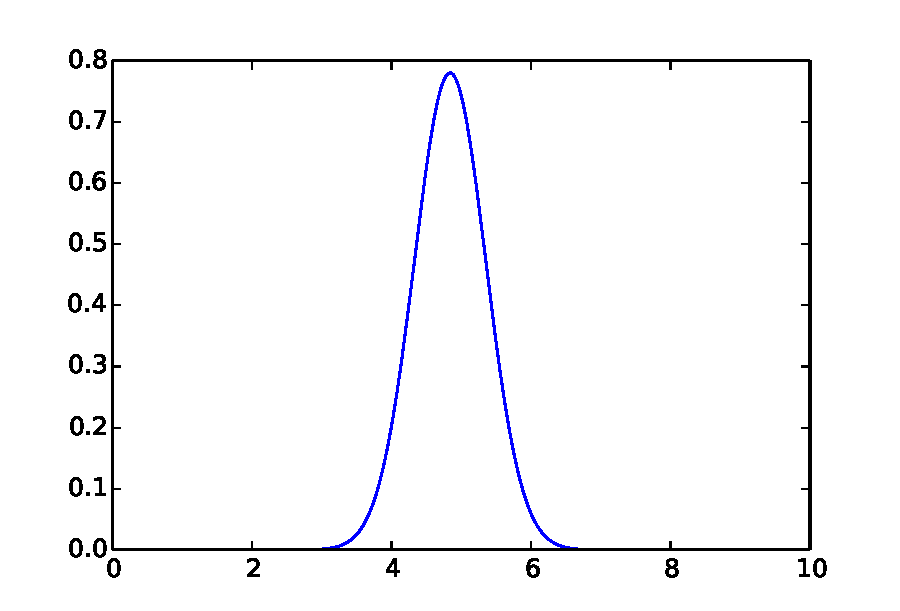
\includegraphics[width=\textwidth]{fig_mu}
      \caption{$q(\mu)$}
    \end{subfigure}
    \begin{subfigure}[b]{0.4\textwidth}
      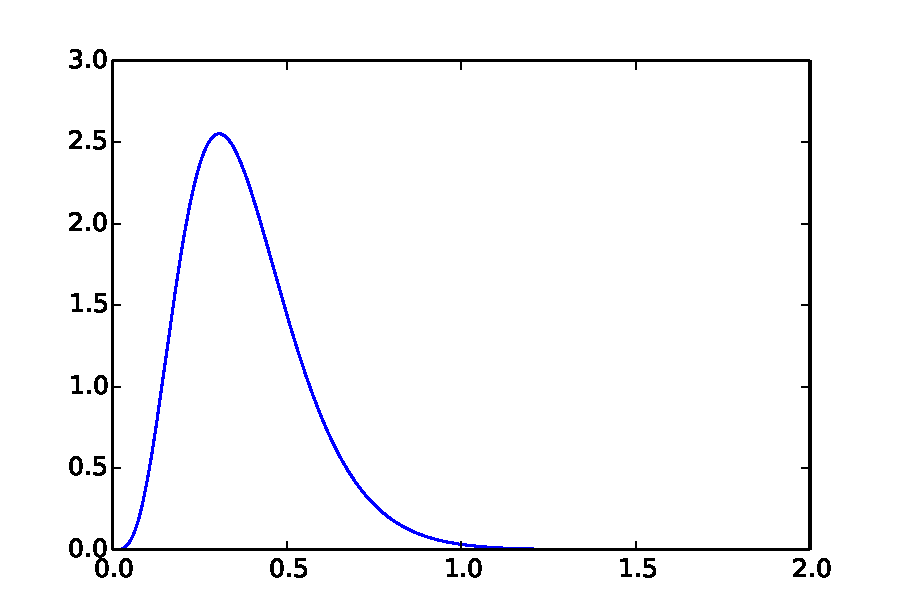
\includegraphics[width=\textwidth]{fig_tau}
      \caption{$q(\tau)$}
    \end{subfigure}
  \end{center}
  \caption{The posterior approximations of $\mu$ and $\tau$.}
  \label{fig:posterior}
\end{figure}

\section{Conclusions}

BayesPy provides a simple and efficient way to construct conjugate exponential
family models and to find the variational Bayesian posterior approximation in
Python.
%
Future plans for BayesPy include implementing more inference engines (e.g.,
maximum likelihood, expectation propagation and Gibbs sampling), improving the
VB engine (e.g., collapsed variational inference \citep{Hensman:2012} and
Riemannian conjugate gradient method \citep{Honkela:2010}) and implementing nodes
for non-parametric models (e.g., Gaussian processes and Dirichlet processes).




% Acknowledgements should go at the end, before appendices and references

%\acks{?}


\vskip 0.2in
\bibliography{bibliography/bibliography.bib}

\end{document}

%%% Local Variables: 
%%% mode: latex
%%% TeX-PDF-mode: t
%%% TeX-master: t
%%% End: 
